%%%%%%%%%%%%%%%%%%%%%%%%%%%%%%%%%%%%%%%%%%%%%%%
% BEGIN ARBEID EN ENERGIE
%%%%%%%%%%%%%%%%%%%%%%%%%%%%%%%%%%%%%%%%%%%%%%%

\chapter{Arbeid en Energie}\label{chap:energie}

In dit hoofdstuk worden arbeid en energie geintroduceerd. Deze zeer belangrijke begrippen
in de klassieke fysica zijn ook voor quantumfysica en relativiteitstheorie van levensbelang. Als
je daarom de klassieke begrippen goed kent, maak je daarmee je introductie in de moderne 
natuurkunde een stuk eenvoudiger.  Verder wordt er in dit hoofdstuk aandacht besteed aan
behoud van energie en in welke gevallen je daarmee op eenvoudige wijze ingewikkelde
problemen kan oplossen.

In Giancoli worden energie en behoud daarvan behandeld in:
\begin{itemize}
\item Hoofdstuk 7
\item Hoofdstuk 8
\end{itemize}

\section{Arbeid en Vermogen}

Arbeid is het eerste belangrijke begrip dat met energie te maken heeft, en aan de hand van
arbeid kunnen we alle vormen van energie exact definieren. In het dagelijks leven heeft het 
begrip arbeid een brede betekenis, maar de natuurkunde zou de natuurkunde niet zijn als
er niet een eenduidige definitie van het begrip arbeid was. Een hoeveelheid arbeid, $\Delta W$,
verricht door een bepaalde kracht $\vec{F}_P$, is gerelateerd aan de hoeveelheid 
verplaatsing, $\Delta x$, in de richting van die kracht:
\begin{equation} 
\Delta W = \vec{F}_P\cdot\vec{\Delta x} 
\end{equation}
De "stip" tussen de kracht en de verplaatsingsvector staat voor het inproduct zoals gedefinieerd
in paragraaf~\ref{sec:vectorcalculus}. Even voor alle duidelijkheid: arbeid is een scalaire grootheid
en gelukkig zorgt het inproduct er voor dat er aan de rechterzijde ook een scalar staat. 
 \begin{figure}[htbp]
\begin{center}
  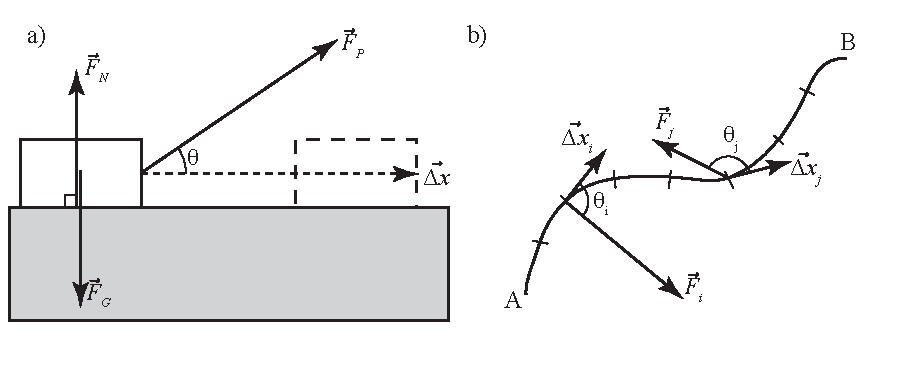
\epsfig{file=Arbeid.pdf, width=\textwidth}
\caption{{\it a) Arbeid in het geval van een constante kracht. b) Arbeid in het algemeen.}}
\label{fig:W}
\end{center}
\end{figure} 
Het inproduct kan ook worden geschreven met behulp van de hoek tussen de kracht en
de verplaatsing zoals getekend in Fig.~\ref{fig:W}~a) als:
\begin{equation}
\Delta W = |\vec{F}_P||\vec{\Delta x}|\cos\theta
\end{equation}
Hieruit zie je onmiddellijk dat de hoeveelheid arbeid alleen afhangt van de component
van de kracht in de richting van de verplaatsing. Wat je ook ziet is dat zowel de zwaartekracht
en normaalkracht in dit specifieke geval geen arbeid verrichten. Hoe wonderlijk het ook 
mag klinken, er hoeft geen arbeid te worden verricht voor verplaatsingen loodrecht op de 
richting van een kracht. Als jij bijvoorbeeld een steen aan een touw boven je hoofd rondslingert, 
verricht je geen arbeid. 

We kunnen het begrip van arbeid meer algemeen definieren voor een willekeurig pad van
A naar B en een willekeurige kracht die als functie van de positie van grootte en richting 
kan veranderen, zoals aangegeven in Fig.~\ref{fig:W}~b). Het enige dat we in dit 
geval moeten doen is het pad opknippen in kleine stukjes aangegeven met $\vec{\Delta x}_i$. 
Vervolgens kan je voor ieder klein stapje uitrekenen hoeveel arbeid de kracht moet
verrichten. Tenslotte moet je alle kleine beetjes bij elkaar optellen om de totale arbeid te
krijgen. Mathematisch kan je dit uiteraard veel korter 'zeggen':
\begin{equation}\label{eq:work_sum}
W = \sum_i \vec{F}_i \cdot \vec{\Delta x}_i = \sum_i |\vec{F}_i||\vec{\Delta x}_i|\cos\theta_i
\end{equation}
Tot nog toe niets verrassend, maar we er zit natuurlijk een onnauwkeurigheid in onze
berekening van $W$, vanwege de eindige stapgrootte $\vec{\Delta x}_i$. We kunnen
nu het aantal stappen naar oneindig laten gaan, terwijl we de stapgrootte oneindig
klein wordt. We kunnen dan de som in vgl.~\ref{eq:work_sum} vervangen door een
integraal (wellicht kennen jullie deze stap al van calculus als de definitie van een integraal):
\begin{equation}\label{eq:defwork}
W = \int_A^B \vec{F}\cdot d\vec{\ell}
\end{equation} 
In het nemen van de limiet hebben we voor alle duidelijkheid $\vec{\Delta x}_i$ vervangen
door $d\vec{\ell}$.
Voor berekenen van de arbeid moet je dus langs je willekeurige pad van A naar B telkens
het inproduct tussen de kracht en de verplaatsing uitrekenen en de resultaten voor elke infinitesimale stap bij elkaar optellen.

\begin{center}
\line(1,0){250}
\end{center}
\begin{voorbeeld} 
Sisyphus houdt ervan dag-in, dag-uit een zware zwerfkei met massa $m$ een helling 
op te duwen. De helling heeft hoogte $h$ en maakt een hoek $\theta$. Om Sisyphus
het niet al te gemakkelijk te maken heeft de helling een coefficient van kinetische
wrijving $\mu_k$.  (i) Hoeveel arbeid moet Sisyphus verzetten om zijn zwerfkei met 
constante snelheid de helling op te duwen? (ii) Bereken hoeveel arbeid elke kracht verzet.
(iii) Wat is de totale hoeveelheid arbeid door alle krachten op de steen?

{\bf Oplossing: }{\it (i) Laten we aannemen dat Sisyphus langs de helling een kracht $\vec{F}_S$ 
uitoefent zoals in Fig.~\ref{fig:sisyphus}. 
 \begin{figure}[htbp]
\begin{center}
  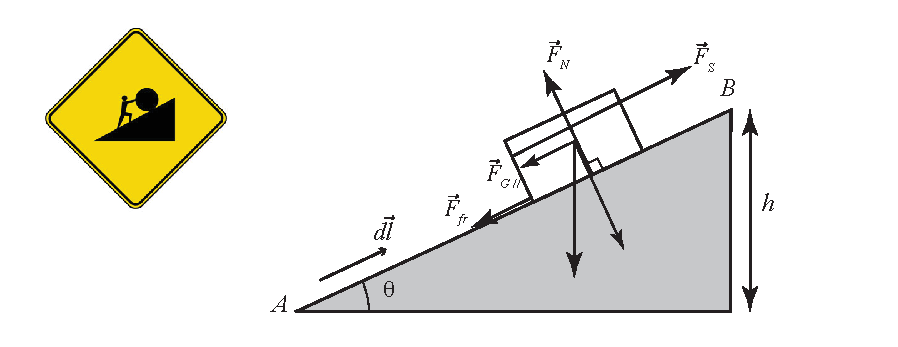
\epsfig{file=Zwerfkei.pdf, width=\textwidth}
\caption{{\it Je moet arbeid leveren om een kei een berg op te duwen.}}
\label{fig:sisyphus}
\end{center}
\end{figure} 
Deze grootte van deze kracht zal gelijk zijn aan de som van alle andere krachten
die parallel aan de helling staan, omdat we een constante snelheid aannemen, $a=0$. Dus:
\begin{eqnarray}
\vec{F}_S & = & \vec{F}_{G\,//}+\vec{F}_{fr} \\
 |\vec{F}_S|  & = & m\,g\,\sin\theta + \mu_k\,m\,g\,\cos\theta 
\end{eqnarray}
Nu we de kracht hebben die Sisyphus moet uitoefenen, kunnen we de arbeid uitrekenen door:
\begin{eqnarray}
W & = & \int_A^B \vec{F}_S \cdot d\vec{\ell} \\
     & = & \int_A^B |\vec{F}_S| |d\vec{\ell}| \\
     & = & (m\,g\,\sin\theta + m\,g\,\mu_k\,\cos\theta)\,L \\
     & = & m\,g\, (\sin\theta + \mu_k\,\cos\theta)\,\frac{h}{\sin\theta} \\
     & = & m\,g\,h + \frac{\mu_k \,m\,g\, h}{\tan\theta}
\end{eqnarray} 
Voor de tweede stap hebben we gebruikt dat het integratiepad langs de helling loopt. De
hoek tussen de kracht $\vec{F}_S$ en $d\vec{\ell}$ is dan $0^{\circ}$. Verder hebben we gebruikt
dat de lengte van de helling is gegeven door $h / \sin\theta$. Je ziet dat de arbeid die
moet worden geleverd bestaat uit een component tegen de zwaartekracht in en een component
tegen de wrijving. (ii) De arbeid die de zwaartekracht heeft verzet is gelijk aan $W_G=-m\,g\,h$ en
de arbeid die de wrijving heeft geleverd is $W_{fr}=-\mu_k \, h / \tan\theta$. In beide gevallen
is de netto verplaatsing tegen de richting van de kracht in. (iii) De totale arbeid van alle
krachten samen is $W=0$, omdat de zwerfkei met constante snelheid beweegt en de totale
kracht dus gelijk is aan $\vec{F}_{tot}=\vec{0}$
}
\end{voorbeeld}
\begin{center}
\line(1,0){250}
\end{center}

Tenslotte is het nog van belang te kijken naar de snelheid waarmee arbeid wordt
geleverd. Als je een zwerfkei de trap op draagt ligt de hoeveelheid arbeid die  je moet
leveren vast, maar je kan ervoor kiezen om langzaam of snel het pad af te leggen. 
Vermogen, $P$, is gedefinieerd als:
\begin{equation}\label{eq:vermogen1}
P = \frac{dW}{dt} 
\end{equation}
We kunnen nu het vermogen relateren aan kracht en snelheid door het volgende 
te schrijven:
\begin{eqnarray}
dW & =  &  \vec{F}\cdot d\vec{\ell} \\
       & \Downarrow & \\
P=\frac{dW}{dt}   & = & \frac{d \vec{F}\cdot d\vec{\ell}}{dt}\\
      & = & \vec{F}\cdot\vec{v}\label{eq:vermogen2}
\end{eqnarray}
Hoewel bovenstaande formule ook wel wiskundig netjes kan worden afgeleid, geldt
dus dat het vermogen gelijk is aan het inproduct van snelheid en kracht.    

\section{Kinetische energie}

Laten we de uitdrukking die we voor de arbeid hebben gevonden eens onder de loep 
nemen. We kunnen de $2^e$ wet van Newton gebruiken om de kracht die voorkomt
in de vergelijking expliciet uit te schrijven:
\begin{eqnarray}
W & = & \int_A^B \vec{F}\cdot d\vec{\ell} \\
    &  = & m\,\int_A^B \frac{d\vec{v}}{dt}\cdot d\vec{\ell} \\
    & = & m\,\int_A^B \frac{d\vec{v}}{dt}\cdot\frac{d\vec{r}}{dt}\,dt \\
    & = & m\,\int_A^B \frac{d\vec{v}}{dt}\cdot\vec{v} \, dt \label{eq:kintmp}
\end{eqnarray}
Let er op dat we het hier hebben over de totale of netto kracht op een object.
We hebben nu een uitdrukking voor de arbeid die zowel de snelheid als de $1^e$ afgeleide 
van de snelheid naar de tijd bevat en die er bovendien tamelijk onsmakelijk uitziet. Maar
laten we nu eerst eens de productregel in gedachten roepen voor differentieren van 
een functie $h(t)=f(t)\,g(t)$. Voor de afgeleide van $f(t)$ naar de tijd krijgen we:
\begin{equation}
\frac{dh}{dt} = f \, \frac{dg}{dt} + \frac{df}{dt}\,g
\end{equation}
Laten we nu een functie $h$ nemen die er uit ziet als:
\begin{equation}
h(t) = f(t) \, f(t)
\end{equation}
Dan geldt voor de afgeleide van $h(t)$ naar de tijd:
\begin{equation}
\frac{dh}{dt} = f\,\frac{df}{dt} + \frac{df}{dt}\,f = 2\,f\frac{df}{dt}
\end{equation}
Dit resultaat gaan we gebruiken om  vgl.~\ref{eq:kintmp} tot de orde te roepen. We kunnen
de laatste regel van vgl.~\ref{eq:kintmp} nu herschrijven als:
\begin{equation}
W = \frac{1}{2}\,m\,\int_A^B\frac{d}{dt} \left( \vec{v} \cdot \vec{v} \right) \,dt
\end{equation}
Deze integraal is uitermate simpel. Je moet namelijk de afgeleide van een functie naar
de tijd integreren over de tijd. Dat geeft niets anders dan de functie zelf:
\begin{equation}
W = \frac{1}{2} \,m\,\left[|\vec{v}|^2\right]_A^B = 
\frac{1}{2}\,m\,|\vec{v}_B|^2 - \frac{1}{2}\,m\,|\vec{v}_A|^2
\end{equation} 
In deze vergelijking stellen de termen aan de rechterkant van de vergelijking de jullie 
welbekende bewegings- of kinetische energie. Dus de netto arbeid op een object leidt tot
een verandering van de kinetische energie, $\Delta K$,  van een object:
\begin{equation}
W = K_2 - K_1 = \Delta K
\end{equation}

\begin{center}
\line(1,0){250}
\end{center}
\begin{voorbeeld} 
Je duwt met kracht $\vec{F}_D$ over een afstand $L$ tegen een object met massa $m$ dat op een
horizontale vloer staat, zonder wrijving. (i) Wat is de kinetische energie na afstand $L$, als de
beginsnelheid nul is? (ii) Wat is de snelheid na afstand $L$?

{\bf Oplossing: }{\it (i) De arbeid die je hebt verricht is:
\begin{equation}
W=\int \vec{F}\cdot\vec{d l} = |\vec{F}_D|\,L= K
\end{equation}
We hebben er gebruik van gemaakt dat het object op een horizontale vloer staat. De zwaartekracht
en de normaalkracht staan loodrecht op de afgelegde weg $d\vec{\ell}$ en leveren dus geen
bijdrage aan de arbeid. 

(ii) De snelheid na afstand $L$ kunnen we oplossen door $K$ gelijk te stellen aan de expliciete
uitdrukking voor de kinetische energie:
\begin{eqnarray}
|\vec{F}_D|\, L & = & \frac{1}{2}\,m\,|\vec{v}|^2 \\
& \Downarrow & \\
|\vec{v}| &  = & \sqrt{\frac{2\,|\vec{F}_D|\,L}{m}}
\end{eqnarray}
Dat is een mooie uitdrukking. Maar wacht nou eens even: dit is een eenparig versnelde 
beweging en daar hadden we in paragraaf~\ref{sec:eenparig} al een uitdrukking gevonden
voor snelheid als functie van de tijd. Wanneer de startsnelheid $\vec{0}$ is geldt:
\begin{equation}\label{ex:attmp}
\vec{v}(t) = \vec{a}\,t
\end{equation}
De versnelling $\vec{a}$ is gelijk aan $\vec{F}_D/m$. Nu moeten we alleen nog even de
tijd uitrekenen die het object over afstand $L$ doet. Dat kunnen we doen door gebruik
te maken van:
\begin{eqnarray}
\vec{r}(t) & = & \frac{1}{2}\,\vec{a}\,t^2 \\
 & \Downarrow & \\
 t & = & \sqrt{\frac{2\,L\,m}{|\vec{F}_D|}}
\end{eqnarray}
Invullen in vgl.~\ref{ex:attmp} - ik zeg doen! - geeft dezelfde uitdrukking voor de eindsnelheid
als die we met de arbeid-energie analyse hebben gevonden. Dit is van groot belang, omdat
we proberen een met zichzelf consistente natuurkunde op te bouwen. Aan de andere kant
is het misschien ook niet al te verrassend dat we hetzelfde antwoord vinden, aangezien
we in beide gevallen zijn uitgegaan van de wetten van Newton (welke?) om tot ons antwoord te
komen.
}
\end{voorbeeld}
\begin{center}
\line(1,0){250}
\end{center}

\section{Conservatieve krachten}

Het blijkt er handig om krachten die we tegenkomen in twee categorie\"{e}n in te delen: 
conservatieve en niet-conservatieve krachten. {\it Een kracht heet conservatief wanneer de arbeid gedaan door
deze kracht door het bewegen van een object van een plek naar een andere onafhankelijk
is van het gekozen pad}. Alle andere krachten zijn niet-conservatief. Een conservatieve 
kracht moet kan slechts afhangen van de positie en niet van andere grootheden als snelheid 
en tijd. 

Laten we eens kijken naar een voorbeeld met zwaartekracht. Stel dat we een massa $m$ langs
een willekeurig pad van $A$ naar $B$ willen brengen waarbij punt $B$ en punt $A$ een
hoogteverschil $h$ hebben. 
 \begin{figure}[htbp]
\begin{center}
  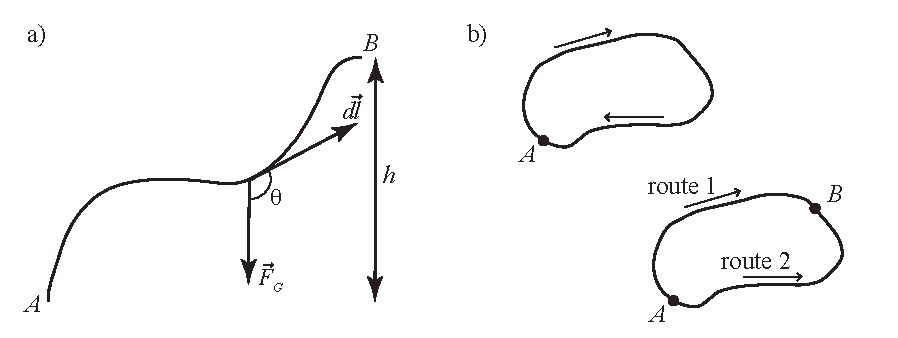
\epsfig{file=Conservatief.pdf, width=\textwidth}
\caption{{\it a) Arbeid door de zwaartekracht. b) Arbeid langs een gesloten pad.}}
\label{fig:conservatief}
\end{center}
\end{figure} 
Dan kunnen we zoals in Fig.~\ref{fig:conservatief} een willekeurig
pad kiezen van $A$ naar $B$ en de arbeid die wordt verricht door de zwaartekracht schrijven
als:
\begin{equation}\label{eq:cons}
W_G = \int_A^B \vec{F}_G\,\cdot\,d\vec{\ell}
\end{equation}
Nu lijkt deze vergelijking op het eerste gezicht duidelijk afhankelijk van het gekozen pad:
immers er komt een pad gedefinieerd door $d\vec{\ell}=(dx,\,dy,\,dz)$ in voor en niets zegt 
mij hoe ik dat pad moet kiezen. Als de zwaartekracht een conservatieve kracht is, zouden 
we moeten kunnen laten zien dat het pad niet uitmaakt. En dat is dit geval eenvoudig: de 
zwaartekracht wordt namelijk gegeven door $\vec{F}_G=(0,\,0,\,-m\,g)$, waardoor  het
inproduct in vgl .~\ref{eq:cons} kan worden uitgewerkt en de vergelijking reduceert tot:
\begin{eqnarray}
W_G & = & \int_A^B (-m\,g)\,dz \\
          & = & -m\,g\,h
\end{eqnarray}
Let op het minteken van de arbeid: de arbeid die door de zwaartekracht is uitgeoefend 
is negatief omdat we punt $B$ boven punt $A$ hebben gekozen. De externe arbeid die is 
uitgeoefend om het object te tillen is uiteraard positief. Het is altijd lastig om bij gedane
arbeid het teken goed te krijgen en te houden.

\begin{center}
\line(1,0){250}
\end{center}
\begin{voorbeeld} \label{ex:cons1}
Een alternatieve definitie van een conservatieve kracht stelt: {\it"Een conservatieve kracht is een 
kracht waarvoor de arbeid rond een willekeurig gesloten pad nul is"}. Bewijs dat dit equivalent
is met de bovenstaande definitie van een conservatieve kracht.

{\bf Oplossing: }{\it Voor dit bewijs rekenen we de arbeid uit langs gesloten pad zoals aangegeven
in Fig.~\ref{fig:conservatief}~b). Dus:
\begin{equation}
W=\int_A^A \vec{F}\cdot\vec{d l}
\end{equation}
Volgens onze alternatieve definitie van een conservatieve kracht zou hier dus nul uit moeten 
komen.  Nu moeten we kijken of er volgens onze originele definitie van een conservatieve kracht 
ook nul uitkomt.

We bekijken daarvoor hetzelfde pad, maar nu opgedeeld in twee etappes: een van $A\rightarrow B$ via 
route~1 en een van $B\rightarrow A$ via route~2. Voor de arbeid van $B\rightarrow A$ langs route~2  
geldt:
\begin{equation}
W_{B\rightarrow A}(\mbox{route~2}) = -W_{A\rightarrow B}(\mbox{route~2})
\end{equation}
Dit volgt direct uit de definitie van de arbeid: als je een pad in tegengestelde richting loopt, dan
verandert $\vec{d l}$ van teken en dus ook de arbeid. Onze originele definitie van een
conservatieve kracht vertelt ons dat de arbeid onafhankelijk is van het gekozen pad, dus:
\begin{equation}
W_{A\rightarrow B}(\mbox{route~1})= W_{A\rightarrow B}(\mbox{route~2})
\end{equation}
Nu kunnen we de arbeid langs het gesloten pad uitrekenen:
\begin{eqnarray}
W_{A\rightarrow A} & = & W_{A\rightarrow B}(\mbox{route 1}) + W_{B\rightarrow A}(\mbox{route~2}) \\
                                   &= & W_{A\rightarrow B}(\mbox{route 1})  - W_{A\rightarrow B}(\mbox{route~2}) \\
                                   & = & W_{A\rightarrow B}(\mbox{route 1})  - W_{A\rightarrow B}(\mbox{route~1}) \\
                                   & = & 0
\end{eqnarray}
Beide definities van conservatieve kracht zijn dus equivalent.
}
\end{voorbeeld}
\begin{center}
\line(1,0){250}
\end{center}
De definitie van een conservatieve kracht zoals in voorbeeld~\ref{ex:cons1} benadrukt
een belangrijk aspect van conservatieve krachten. De arbeid die door een conservatieve
kracht wordt gedaan is herbruikbaar: langs een gesloten pad worden alle stukken met
positieve arbeid gecompenseerd door stukken waar de arbeid negatief is. In het geval
van de zwaartekracht moet jij arbeid uitoefenen als je iets omhoog beweegt, die je kan
terugwinnen door hetzelfde object weer naar beneden te laten gaan. Vandaar ook de
naam 'conservatieve kracht', wat niets met de politieke voorkeur van een kracht te maken
heeft maar wel met het feit dat er iets 'behoudends' aan is.

Belangrijke voorbeelden van conservatieve krachten zijn de zwaartekracht, elektrische krachten,
en krachten uitgeoefend door veren en elastieken (die we later tegen gaan komen). 
Wrijvingskrachten daarentegen zijn niet-conservatief. Dat voel je natuurlijk al wel aan, aangezien
bij bijvoorbeeld het verschuiven van een zware bank in je kamer, het er wel degelijk toe doet
hoe je va $A$ naar $B$ gaat. Een langere weg betekent dat er meer arbeid moet worden gedaan, 
wat niet zo gek is voor een kracht die altijd tegengesteld staat aan de richting waarin je een
object beweegt. Andere voorbeelden van niet-conservatieve krachten zijn bijvoorbeeld
luchtwrijving en voortstuwing door raketten, motoren of mensen. 

\begin{center}
\line(1,0){250}
\end{center}
\begin{voorbeeld} \label{ex:veer1}
De kracht die een veer uitoefent als deze wordt uitgerekt of ingedrukt, wordt gegeven door 
de wet van Hooke. Deze vertelt dat de veerkracht, $F_V$, als functie van uitrekking of compressie 
wordt gegeven door:
\begin{equation}
F_V = -k\,(x -x_0)
\end{equation}
Hierbij is $k$ de veerconstante, $x-x_0$ de uitrekking of compressie, met $x_0$ de evenwichtspositie. Voor 
het gemak gaan we eens in 1-D iets uitrekenen, omdat de veren in dit college maar in 1~richting zullen worden 
ingedrukt. Bewijs dat de veerkracht conservatief is.

{\bf Oplossing: }{\it Om te bewijzen dat de veerkracht conservatief is, moeten we de arbeid van het uitrekken of indrukken
van willekeurige positie $x_A$ naar $x_B$. Dus:
\begin{eqnarray}
W & =  & \int_{x_A}^{x_B} F_V \, dx  \\
    & =  & -\frac{1}{2}\,k\,((x_B-x_0)^2 - (x_A-x_0)^2)
\end{eqnarray}
De arbeid hangt alleen af van het begin en eindpunt, en is niet afhankelijk van het gekozen pad. De 
veerkracht is dus conservatief.
}
\end{voorbeeld}
\begin{center}
\line(1,0){250}
\end{center}

\section{Potentiele energie}

In de vorige paragraaf hebben we de arbeid die een conservatieve kracht uitoefent bekeken en
gezien dat deze arbeid onafhankelijk is van het gekozen pad van $A\rightarrow B$ en alleen
afhangt van de coordinaten van het eind- en beginpunt van ons pad. We kunnen nu voor 
een conservatieve kracht een nieuwe grootheid definieren die we potentiele energie $U$ noemen.
Verschillen in potentiele energie zijn gedefinieerd als:
\begin{equation}
\Delta U = U_2 - U_1 \equiv -\int_1^2\vec{F}\cdot d\vec{\ell} 
\end{equation}
Een dergelijk verschil in potentiele energie behorend bij een conservatieve kracht geeft aan wat
voor potentie die kracht heeft om arbeid te verrichten. Let op dat potentiele energie alleen betekenis heeft
als je te maken hebt met een conservatieve kracht: voor een niet conservatieve kracht zoals wrijving hangt 
de arbeid af van het gekozen pad, en is $\Delta U$ niet eenduidig.

Als je bijvoorbeeld een zwerfkei met massa $m$ een afstand $h$ van de grond krijgt, dan
heeft deze steen een potentiele energie van $U = m\,g\,h$. Dit is de hoeveelheid arbeid die
jij - of Sisyphus - moet leveren om de zwerfkei op te tillen. Wanneer je de steen laat vallen wordt 
er weer precies een hoeveelheid arbeid $W=m\,g\,h$ geleverd door de zwaartekracht (potentiele
energie wordt omgezet in bewegingsenergie).  Nog even voor alle duidelijkheid. als je spreekt
over potentiele energie, bedoel je de potentiele energie die een object heeft in de aanwezigheid
van een bepaalde conservatieve kracht.

Nu is het vaak zo dat niet de kracht zelf, maar de potentiele energie als functie van positie
wordt gegeven. Dan kan je je afvragen of je de relatie kan vinden tussen die potentiele energie
en de bijbehorende kracht. Het antwoord is ja. Als we eerst een in 1-D kijken naar de uitdrukking
voor de potentiele energie, dan kunnen we stellen:
\begin{equation}
U(x) = -\int F(x)\,dx + C
\end{equation}
Als we nu kiezen:
\begin{equation}
F(x) = -\frac{dU(x)}{dx}
\end{equation}
Hieruit zie je dat de afgeleide van de potentiele energie naar de positie inderdaad precies de bijbehorende
kracht voorstelt. Als je een potentiele energie hebt die snel verandert als functie van de plaats is de 
kracht groot en vice-versa. Het beste kan je potentiele energie voorstellen als een heuvel met steile en minder steile
hellingen, waarbij de kracht die je moet leveren om de heuvel te beklimmen het grootst
is waar de helling het steilst is. De relatie tussen potentiele energie en kracht klopt dus met je intuitie.

Om de boel compleet te maken: voor een potentiele energie die afhangt van $(x,\,y,\,z)$ is de relatie 
tussen kracht en potentiele energie gegeven door de 3-D versie van een afgeleide:
\begin{equation}
\vec{F} = -\ihat \frac{\partial U}{\partial x} -\jhat \frac{\partial U}{\partial y} -\khat \frac{\partial U}{\partial z} 
\end{equation}
De partiele afgeleide, $\partial /\partial x$, staat voor de afgeleide naar $x$ met $y$ en $z$ constant.
In volgende vakken zullen jullie deze 3-D afgeleide nog vaak tegenkomen. Hij heet de gradient, $\vec{\nabla}$, en 
met de gradient kan de bovenstaande afgeleide worden geschreven als:
\begin{equation}
\vec{F} = -\vec{\nabla} U
\end{equation}

\section{Behoud van energie}

We hebben in de voorafgaande paragrafen twee vormen van energie ontmoet: kinetische
energie
en voor conservatieve krachten potentiele energie. Beide vormen van energie zijn gerelateerd
aan het begrip arbeid dat we in de eerste paragraaf van dit hoofdstuk zijn tegengekomen.
Door het combineren van kinetische en potentiele energie in conservatieve systemen, d.w.z 
systemen waar alleen conservatieve krachten arbeid verzetten, komen we op een van de 
belangrijkste behoudswetten in de klassieke natuurkunde: namelijk behoud van mechanische
energie. Als we 
kijken naar de som van de verandering van kinetische- en potentiele energie, dan
krijgen we:
\begin{eqnarray}
\Delta~K + \Delta~U & = & W_{netto}-W_{netto} \\
                                     & = & 0 \\
                                     & \Downarrow & \\
\frac{1}{2}\,m\,|\vec{v}_1|^2 + U_1 & = & \frac{1}{2}\,m\,|\vec{v}_2|^2+U_2
\end{eqnarray}
In het geval er alleen conservatieve krachten werken, is de som van kinetische energie
en potentiele energie, ofwel de totale energie $E_{tot}$ constant:
\begin{equation}
E_{tot} = K + U
\end{equation}

\begin{center}
\line(1,0){250}
\end{center}
\begin{voorbeeld} 
Bewijs dat energie behouden is door het expliciet berekenen van de tijdsafgeleide van de totale energie. (Doe maar in 1-D)

{\bf Oplossing: }{\it Als de totale energie behouden is, moet dus gelden:
\begin{equation}
\frac{dE_{tot}}{dt} = 0
\end{equation}
We kunnen in 1-D schrijven:
\begin{eqnarray}
\frac{dE_{tot}}{dt} & = & \frac{d}{dt}\left(\frac{1}{2}\,m\,v_x^2+U(x)\right) \\
                                & = & m\,v_x\,\frac{d v_x}{dt} + \frac{dU}{dt} \\
                                & = & m\,v_x\,a_x + \frac{dx}{dt}\frac{dU}{dx} \\
                                & = & v_x\,\left(m\,a_x - F_x\right) \\
                                & = & 0
\end{eqnarray}
We hebben gebruikt dat $F_x=-dU/dx$ en in de laatste stap hebben we simpelweg
de $2^e$ wet van Newton gebruikt. Het concept van energiebehoud dat we dus in deze
paragraaf hebben geintroduceerd, volgt in feite direct uit de wetten van Newton. Klassieke
mechanica zit wat dat betreft natuurlijk mooi consistent in elkaar.
} 
\end{voorbeeld}
\begin{center}
\line(1,0){250}
\end{center}

Als er naast conservatieve krachten ook nog niet-conservatieve krachten zoals
wrijving in het spel zijn, dan neemt de hoeveelheid mechanische energie in het systeem af als 
functie van de tijd. Een deel, en meestal alle energie wordt dan uiteindelijk gedissipeerd in
de vorm van warmte. Maar denk er wel om dat de totale energie
nog steeds behouden is: de mechanische energie wordt alleen omgezet in een vorm die
niet meer mechanisch van aard is. We kunnen de wet van behoud van mechanische
energie dan ook eenvoudig algemeen geldig maken, door er een extra term aan toe te voegen:
\begin{equation}
\Delta~K+\Delta~U +\Delta~E_{rest} = 0
\end{equation}
De term $\Delta~E_{rest}$ bevat alle vormen van energie die niet mechanisch van aard zijn.
Voor zover we weten is de wet van behoud van totale energie universeel geldig in de natuurkunde.
Er zijn tot op vandaag geen processen gevonden die de wet van behoud van energie schenden. 
Dat maakt deze wet ook tot een enorm krachtig gereedschap voor het analyseren van 
problemen. Zeker als er alleen conservatieve krachten in het spel zijn, is het oplossen
van problemen vaak een stuk eenvoudiger met behoud van energie, dan met de $2^e$ wet
van Newton, hoewel de resultaten natuurlijk hetzelfde moeten zijn.

\begin{center}
\line(1,0){250}
\end{center}
\begin{voorbeeld} 
Een slinger met lengte $l$ en massa $m$ staat op $t=0$ stil met uitwijking $\theta(t=0)=\theta_0$ zoals
in Fig.~\ref{fig:energiebehoud1}~a). Wat is de snelheid van de de massa bij uitwijking $\theta$?
 \begin{figure}[htbp]
\begin{center}
  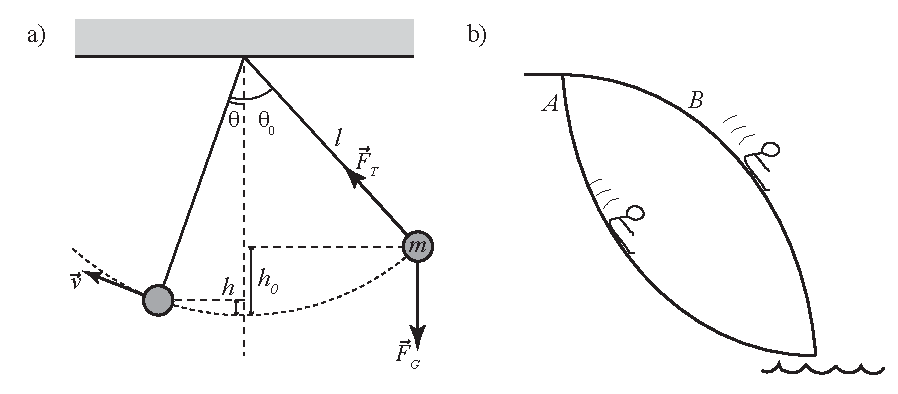
\epsfig{file=EnergiebehoudVoorbeeld.pdf, width=\textwidth}
\caption{{\it a) Slinger. b) Glijbaan}}
\label{fig:energiebehoud1}
\end{center}
\end{figure} 

{\bf Oplossing: }{\it Laten we beginnen te kijken naar de krachten die voor de slinger relevant zijn. Je
hebt de zwaartekracht, $\vec{F}_G$, op de massa en de spankracht, $\vec{F}_T$ in het touw. De zwaartekracht
is conservatief en de spankracht niet, maar toch geldt behoud van energie, omdat de spankracht geen
arbeid verricht. De spankracht staat namelijk altijd loodrecht op de bewegingsrichting van de massa.
Omdat alleen de zwaartekracht arbeid verricht kunnen we dus concluderen dat:
\begin{equation}
E = T+U = \mbox{constant}
\end{equation}
Bij het loslaten van de slinger is de snelheid $\vec{v}(t=0)=\vec{0}$ dus de massa heeft alleen potentiele
energie. Voor het uitrekenen van de potentiele energie kiezen we als de positie van de massa
voor $\theta=0$ als nulpunt. Dus voor $\theta=\theta_0$ geldt voor de potentiele energie:
\begin{equation}
U(\theta=\theta_0) = m\,g\,l\,(1-\cos\theta_0)
\end{equation}
Aangezien energie behouden is kunnen we nu de grootte van de snelheid voor een willekeurige hoek 
$\theta$ uitrekenen, door energiebehoud te gebruiken:
\begin{eqnarray}
E(\theta_0) & = & E(\theta) \\
m\,g\,l\,(1-\cos\theta_0)  & = & \frac{1}{2}\,m\,|\vec{v}|^2 + m\,g\,l\,(1-\cos\theta)  \\
  & \Downarrow & \\
|\vec{v}| &= &\sqrt{2\,g\,l\,(\cos\theta-\cos\theta_0)}  
\end{eqnarray}
Je ziet dat de snelheid onafhankelijk is van de massa en alleen afhangt van $l$, $g$ en de de beide hoeken.
Verder zie je dat je alleen de grootte van de snelheid op deze manier hebt berekend. In het geval van een
slinger kan de massa zowel met de klok mee als tegen de klok in hoek $\theta$ passeren.
} 
\end{voorbeeld}

\begin{center}
\line(1,0){250}
\end{center}

\begin{voorbeeld} 
In het zwembad zijn twee glijbanen  $A$ en $B$ zoals getekend in 
Fig.~\ref{fig:energiebehoud1}~b). De glijbanen zijn even lang en je kan zonder
wrijving naar beneden glijden. (i) Wat is de eindsnelheid die je hebt aan de bodem van 
beide glijbanen? (ii) Bij welke glijbaan bent je het eerst beneden?

{\bf Oplossing: }{\it (i) In beide gevallen is er een zelfde hoeveelheid gravitationele potentiele energie
veranderd in kinetische energie, terwijl de normaalkracht op de zwemmer geen arbeid heeft verricht. De
eindsnelheid van beide zwemmers is gelijk. (ii) Glijbaan $A$ ligt in zijn geheel onder glijbaan $B$. Op glijbaan
$A$ wordt er eerder potentiele energie omgezet in kinetische energie, en heb je dus gemiddeld een hogere
snelheid.} 
\end{voorbeeld}


\begin{center}
\line(1,0){250}
\end{center}


\begin{voorbeeld} \label{ex:achtbaan}

Een karretje glijdt zonder wrijving vanaf hoogte $h$ in een looping met straal $R$. Bij het
loslaten op $t=0$ is de snelheid van het karretje $\vec{v}(t=0)=\vec{0}$. (i) Wat is de minimale hoogte $h=h_{min}$ zodat het karretje (met docent Colijn) door de looping heen komt zonder uit
de baan te vallen (zie punt\,2 in Fig.~\ref{fig:achtbaan})? (ii) Druk de normaalkracht in punt\,1 
uit in termen van $h$ en $R$. (iii) Hoe groot is de kracht die je ondervindt op punt~1 als je op
de hoogte gevonden bij (i) begint?
 \begin{figure}[htbp]
\begin{center}
  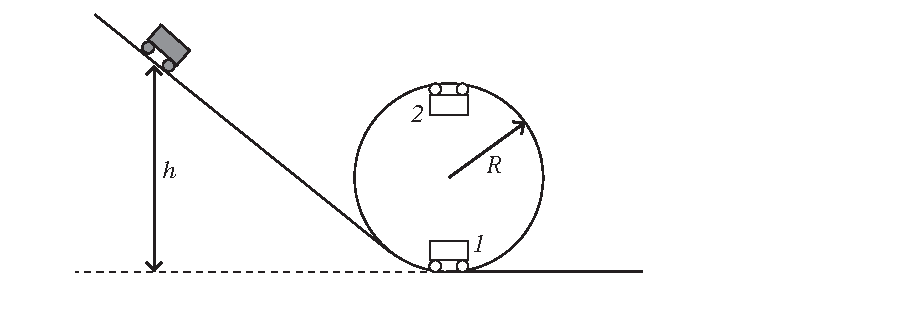
\epsfig{file=Achtbaan.pdf, width=\textwidth}
\caption{{\it Achtbaan}}
\label{fig:achtbaan}
\end{center}
\end{figure} 

{\bf Oplossing: }{\it (i) We moeten gebruik maken van energiebehoud en van hetgeen we
weten over een cirkelbeweging. Als we een krachtenanalyse maken in het punt\,2  
(teken de krachten zelf) dan zie je dat:
\begin{equation}
\vec{F}_G+\vec{F}_N = \vec{F}_C
\end{equation}
Ofwel de som van de zwaartekracht en de normaalkracht moet gelijk zijn aan de centripetaalkracht
die hoort bij het door de looping gaan. Maar de vraag is te kijken naar het geval waarbij 
het karretje net in de looping blijft: dus waarvoor geldt $\vec{F}_N = \vec{0}$. In dat geval geldt:
\begin{eqnarray}
m\,g & = & \frac{m\,|\vec{v}|^2}{R} \\
& \Downarrow & \\
|\vec{v}| & =  & \sqrt{g \, R}
\end{eqnarray}

Nu kunnen we gebruik maken van de wet van behoud van energie om te kijken wat de minimale hoogte is waarbij deze snelheid nog wordt gehaald:
\begin{eqnarray}
E(t=0)& = & E(\mbox{{\it punt 2}}) \\
m\,g\,h_{min} & = & \frac{1}{2}m\,|\vec{v}|^2 + 2\,m\,g\,R \\
& \Downarrow & \\
h_{min} & = & \frac{5}{2} R
\end{eqnarray}
Dus als je een object door een looping laat glijden met straal $R$, moet je tenminste 
vanaf een hoogte van $2.5\times$ komen om door het hoogste punt van de looping
te komen.

(ii) De normaalkracht die op je wordt uitgeoefend beneden in de looping op punt\,1 is 
de som van de centripetaalkracht en de normaalkracht ten gevolge van de zwaartekracht:
\begin{eqnarray}
\vec{F}_N & = & -\vec{F}_G +\vec{F}_C \\
& = & \left(m\,g + \frac{m\,|\vec{v}|^2}{R}\right)\khat
\end{eqnarray}
Verder weten we de snelheid in punt\,1uit energiebehoud:
\begin{eqnarray}
m\,g\,h & = & \frac{1}{2}m\,|\vec{v}|^2\\
&\Downarrow&\\
|\vec{v}| & = & \sqrt{2\,g\,h}
\end{eqnarray}
Invullen in de eerste vergelijking levert:
\begin{equation}\label{eq:exloop}
\vec{F}_N = m\,g\left(1 + \frac{2\,h}{R}\right) 
\end{equation}
Dus je 'gewicht' neemt toe als je door de bocht gaat. Dit weten jullie natuurlijk allang.

(iii) Als je de looping net haalt dan gold $h=\frac{5}{2}R$ en dit kunnen we invullen
in vgl.~\ref{eq:exloop} en dan krijgen we op punt\,1 in de looping:
\begin{equation}
\vec{F}_N  = 6\,m\,g\,\khat
\end{equation}
Je bent dan dus $6\times$ zo zwaar als normaal!
}
\end{voorbeeld}

\begin{center}
\line(1,0){250}
\end{center}

\section{Wat moet ik weten en kunnen?}

Als je dit hoofdstuk hebt bestudeerd moet je weten:
\begin{itemize}
\item Wat is arbeid, kinetische- en potentiele energie.
\item Wat is een conservatieve kracht? Wat zijn voorbeelden van dergelijke krachten?
\item Wat is een niet-conservatieve kracht? Wat zijn voorbeelden van dergelijke krachten?
\item Behoud van energie in het algemeen.
\item Behoud van mechanische energie, als er alleen conservatieve krachten werken.
\end{itemize}
En je moet kunnen:
\begin{itemize}
\item Arbeid uitrekenen.
\item Kinetische en potentiele energie uitrekenen.
\item Behoud van energie gebruiken om problemen op te lossen.
\end{itemize}

\section{Opdrachten}

\begin{enumerate}
\item Giancoli hoofdstuk 7: 1, 6, 11, (16 - 25), 33, 35, 42, 43, 45, 46, 57, 60, 61, 63, 64, 68, 75, 79, 86, 90, 91 
\item Giancoli hoofdstuk 8: 7, 8, 9, 17, 21, 22, 23, 28, 36, 42, 83, 84, 85, 86, 87, 92 
\item Wat is de eenheid van arbeid? En van kinetische en potentiele energie?
\item Leg uit waarom wrijving geen conservatieve kracht kan zijn.
\item Leg uit waarom een conservatieve kracht niet kan afhangen van snelheid.
\item Kijk nog eens naar voorbeeld~\ref{ex:achtbaan}. Wat gebeurt er met $h_{min}$ als
de wrijving ongelijk 0 is? Stel dat de wrijvingscoefficient voor glijdende wrijving gegeven
is door $\mu_k$. Wat moet je doen om $h_{min}$ te vinden? Heb je genoeg informatie, 
of niet? Leg je antwoord uit.
\end{enumerate}

